\documentclass[11pt,letter,oneside]{report}
\usepackage[pdftex]{graphicx}
\begin{document}

\title{Space Invaders}
\author{Peter Hamilton and Jared Pilcher}
\date{Fall 2011}
\maketitle

\tableofcontents

\chapter{Space Invaders Overview}
\section{History of Space Invaders}

Space invaders was a really popular game in the early 16th century.  Children played it out in the fields with the trebuchet when their parents were out of town.

Designed by Tomohiro Nishikado, Space Invaders is one of the greatest arcade games of all time.  It hold the Guinness World Record for greatest arcade game.
 

\section{Game Play}

\subsection{Objective}

The world is being invaded by marching aliens.  All of humanity has gathered behind 4 bunkers for protection.  You control the only weapons available, a supply of 3 tanks and a handful of missiles. Kill all the aliens! Watchout! The alien mothership flies over head! Destroy it at all costs!  The fate of the world rests in your hands...

\subsection{The Tank}
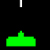
\includegraphics[]{tank.jpg}

You are the tank. Push the left button to move left, and the right button to move right. 

Watchout! Enemy fire rains from above! Dodge the alien fire by moving the tank left or right. 

Fire your missile to destroy the alien invaders! Push the middle button to fire your missile, aiming for the aliens. When the missile hits an alien, it dies. Be careful! They move left and right, and get closer as time goes on.

\subsection{Enemies}

\subsubsection{Spaceship}

The alien mothership circles the Earth, looking for its prey. Destroy it at all costs! It flies occasionally from left to right. As it flies overhead, launch your tank missile by pushing the middle button. Be careful, it tries to evade you missile, so shoot accurately and quick!


\includegraphics[]{big-alien.png}

\subsubsection{Aliens}
55 aliens are marching toward your position! You are charged with destroying all of them before they reach you! Fire your missiles to kill them!There are 55 aliens on the screen.

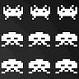
\includegraphics[]{aliens.jpg}

\subsection{Points}

\section{Game Details and Specifications}

\subsection{Aliens}

\subsection{The Tank}

\subsection{Bullets}

\chapter{Bug Reports and File Organization}

\section{Bug Reports}

\subsection{Drawing Bullets}

\end{document}
